% Structure follows unpacked-paper/exp.tex fig:exp5-m (417--472):
% 0.8\linewidth legend, \vspace{-2ex}, 0.33\columnwidth cells, \hspace{-2.5ex},
% a blank line between the two rows. Image paths and short titles differ.
% Not the missing 3D k-sweep float. Heights are synthetic.
\begin{figure*}[t]
  \centering

  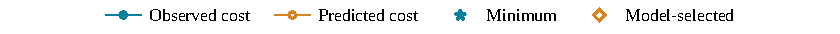
\includegraphics[width=0.8\linewidth]{e2-legend.pdf}

  \vspace{-2ex}

  \subfigure[Syn-A, LT, Full]{
      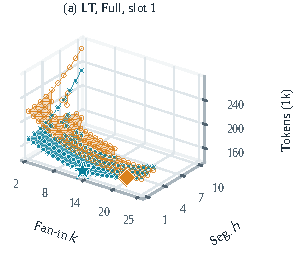
\includegraphics[width=0.33\columnwidth]{panels/p01.pdf}
  }
  \hspace{-2.5ex}
  \subfigure[Syn-B, LT, Full]{
      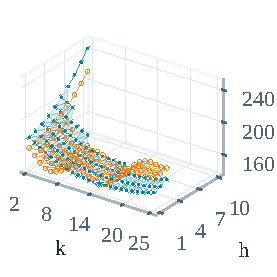
\includegraphics[width=0.33\columnwidth]{panels/p02.pdf}
  }
  \hspace{-2.5ex}
  \subfigure[Syn-C, LT, Full]{
      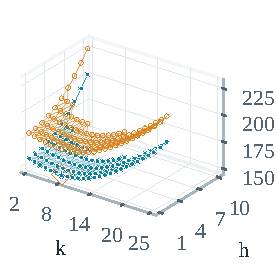
\includegraphics[width=0.33\columnwidth]{panels/p03.pdf}
  }
  \subfigure[Syn-D, LT, LIMIT10]{
      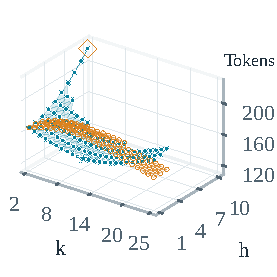
\includegraphics[width=0.33\columnwidth]{panels/p04.pdf}
  }
  \hspace{-2.5ex}
  \subfigure[Syn-E, LT, LIMIT10]{
      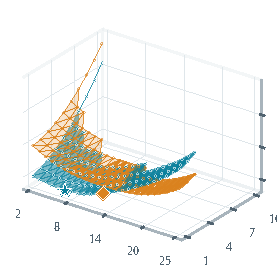
\includegraphics[width=0.33\columnwidth]{panels/p05.pdf}
  }
  \hspace{-2.5ex}
  \subfigure[Syn-F, LT, LIMIT10]{
      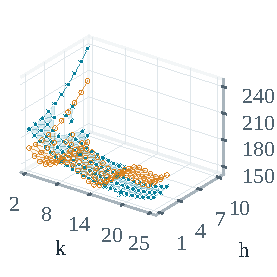
\includegraphics[width=0.33\columnwidth]{panels/p06.pdf}
  }

  \subfigure[Syn-G, SW, Full]{
      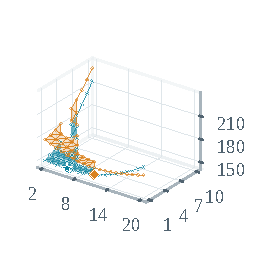
\includegraphics[width=0.33\columnwidth]{panels/p07.pdf}
  }
  \hspace{-2.5ex}
  \subfigure[Syn-H, SW, Full]{
      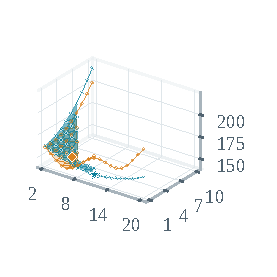
\includegraphics[width=0.33\columnwidth]{panels/p08.pdf}
  }
  \hspace{-2.5ex}
  \subfigure[Syn-I, SW, Full]{
      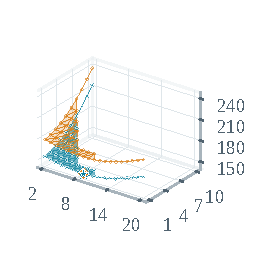
\includegraphics[width=0.33\columnwidth]{panels/p09.pdf}
  }
  \subfigure[Syn-J, SW, LIMIT10]{
      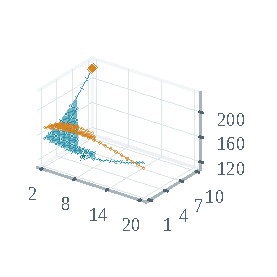
\includegraphics[width=0.33\columnwidth]{panels/p10.pdf}
  }
  \hspace{-2.5ex}
  \subfigure[Syn-K, SW, LIMIT10]{
      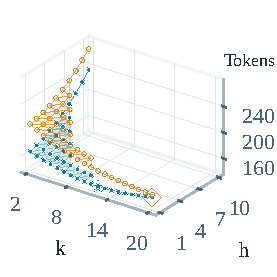
\includegraphics[width=0.33\columnwidth]{panels/p11.pdf}
  }
  \hspace{-2.5ex}
  \subfigure[Syn-L, SW, LIMIT10]{
      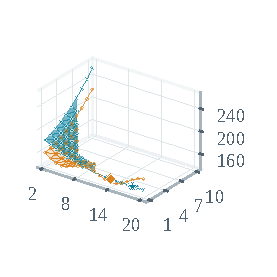
\includegraphics[width=0.33\columnwidth]{panels/p12.pdf}
  }

  \caption{Synthetic schematic cost (tokens $\times 10^{3}$), not experimental results.}
  \label{fig:e2-surface-exp5-12}
\end{figure*}
